% Provenance (never printed): see sources/outline_sources.md (Year 1: decay systems K-Ar,
% Rb-Sr, U-Pb and radiocarbon; closure temperature; dating sedimentary sequences with
% volcanic ashes; calibrating the scale). Exercise and problem values in the Book 3
% scratch calculator calc/ch25.py; figures from figdata/bachelor-1/decay_curves.py,
% isochron.py and radiocarbon.py (IntCal20, dataset bachelor-1-intcal20).
% The decay law, half-life and decay constant belong to the physics series (recalled);
% the closed system and the isochron of minerals are Book 2's (g12 age-of-the-earth),
% re-founded here with whole-rock samples and least squares. The concordia diagram and
% thermochronology are the Year 3 volume's: prose pointers only. Mass spectrometry is
% the chemistry series' (recalled). The isochron figure uses an invented rhyolite so that
% the Varden granite of the problem is not solved in the course.
\chapter{طرائق التأريخ الإشعاعي}\label{ch:b1:radiometric-methods}

في عام 2001 أبلغ فريق عمل على حبيبات فُتاتية من الزركون من تلال جاك في غرب أستراليا عن واحدة تبلّرت قبل \num[uncertainty-mode=separate]{4404 \pm 8} مليون سنة. وأكّدت أعمال لاحقة عمر هذه الحبيبات: إنها أقدم مادة معروفة من أيّ نوع تكوّنت على الأرض، وتبيّن أن \omterm{def:b1:layered-earth:layers}{قشرة} تكوّنت في غضون نحو 160 مليون سنة من ولادة المجموعة الشمسية. وعلى الطرف الآخر من السلّم، وضعت أعمار الأرغون الانقراض عند نهاية الطباشيري قبل \qty{66.00}{\Ma}، في غضون \num{32000} سنة من الصدمة التي يُعتقد أنها سبّبته. وكلا الرقمين يأتيان من عدّ الذرّات: أصلٌ مشعّ يضمحلّ بمعدّل معلوم، وابنةٌ تتراكم. ويشرح هذا الفصل كيف تُقرأ هذه الساعات، ولماذا يؤرّخ كل منها حدثًا مختلفًا، وكيف تعلّق مخطّط \cref{ch:b1:stratigraphic-scale} على مقياس بالسنين.
% ledger: wilde01:4404, uw14:jack-hills, ics:base.Paleogene, renne:kpg

\begin{omfigure}
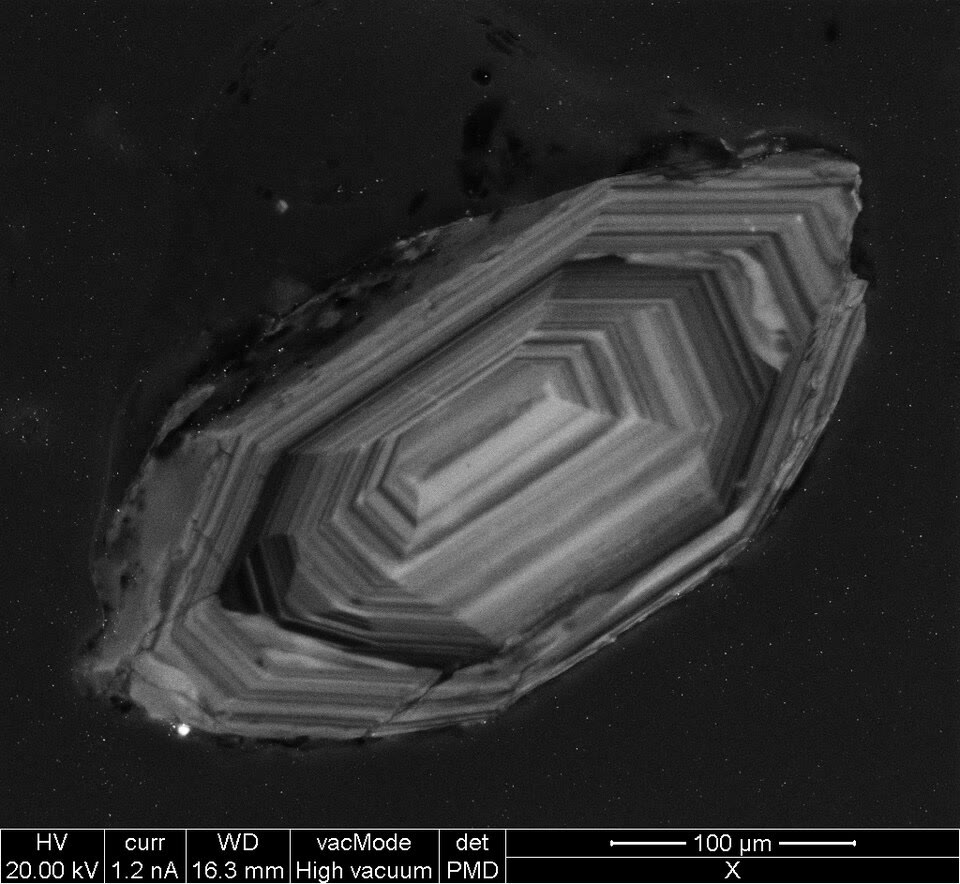
\includegraphics[width=0.5\linewidth]{images/book3/b1-zircon-cl.jpg}

{\small حبّة من الزركون، طولها نحو ثلث مليمتر، مُصوَّرة بالضوء الذي تُصدره تحت شعاع الإلكترون في مجهر إلكتروني ماسح (التألّق الكاثودي). والنطاقات التي تتبع أوجه البلّورة مناطق ذات تركيب مختلف قليلًا، رُسّبت واحدة بعد أخرى أثناء نموّها. وقد التُقطت الحبّة من حجر رملي، فهي أقدم من الحجر الرملي: إنها تؤرّخ الصخر الذي تآكلت منه. (Emmanuel Roquette, CC~BY-SA~4.0, عبر Wikimedia Commons.)}
\label{fig:b1:radiometric-methods:zircon}
\end{omfigure}
% ledger: commons:zircon-cl

\begin{recall}
تصف الكتب الفيزيائية الاضمحلال الإشعاعي: تضمحلّ أنوية النظير المشع عشوائيًّا، مستقلّةً عن درجة الحرارة والضغط، فيبقى منها $N$ بعد الزمن $t$ وفق $N = N_0\,e^{-\lambda t}$، حيث $\lambda$ ثابت الاضمحلال؛ ونصف العمر $T = \ln 2/\lambda$. ونظائر العنصر الواحد لها العدد نفسه من البروتونات وأعداد مختلفة من النيوترونات؛ وتصف كتب الكيمياء مطياف الكتلة الذي يفرز الأيونات بحسب كتلتها. وفي الكتاب الثاني، الصف الثاني عشر، يكون الصخر أو \omterm{def:b1:rock-forming-minerals:mineral}{المعدن} الذي لم يتبادل ذرّات أصل أو ابنة مع محيطه نظامًا مغلقًا، وقد أعطت \omterm{def:b1:rock-forming-minerals:mineral}{معادن} جرانيت فاردن، حين رُسمت على خطّ \omterm{def:b1:radiometric-methods:isochron}{الإيزوكرون} للروبيديوم–السترونتيوم، عمرًا قدره 310 مليون سنة. والبيوتايت والموسكوفيت والهورنبلند هي \omterm{def:b1:rock-forming-minerals:groups}{الميكا} \omterm{def:b1:rock-forming-minerals:groups}{والأمفيبول} في \cref{def:b1:rock-forming-minerals:groups}. ويمكن استكمال عمر بين مستويين مؤرّخين (\cref{prop:b1:stratigraphic-scale:interpolation}).
\end{recall}
% ledger: tulane:radiometric, villa22:rb87

\section{أنظمة الاضمحلال}\label{sec:b1:radiometric-methods:systems}

تحتاج الساعة إلى عدّين: ما بقي من الأصل، وكمية الابنة التي صنعها منذ بدأت الساعة.

\begin{definition}[الأصل المشعّ، والابنة الإشعاعية]\label{def:b1:radiometric-methods:radiogenic}
في نظام اضمحلال يُستعمل للتأريخ، يكون \emph{الأصل}\index{الأصل المشع} هو النظير المشع الذي يصنع اضمحلاله الساعة، والابنة هي النظير الذي ينتجه اضمحلاله. و\emph{الابنة الإشعاعية}\index{الابنة الإشعاعية}، ويُكتب $D^*$، هي الجزء من الابنة الذي صنعه اضمحلال الأصل داخل العيّنة منذ بدأت الساعة؛ أما الباقي، $D_0$، فكان موجودًا منذ البداية. وعدد ذرّات الابنة التي تُقاس اليوم هو $D = D_0 + D^*$.
\end{definition}

\begin{proposition}[النموّ الإشعاعي ومعادلة العمر]\label{prop:b1:radiometric-methods:growth}
في نظام مغلق يحتوي $P$ ذرّة من الأصل اليوم، فإن \omterm{def:b1:radiometric-methods:radiogenic}{الابنة الإشعاعية} التي تُصنع في زمن $t$ هي
\[
  D^* = P\,\bigl(e^{\lambda t} - 1\bigr),
\]
بشرط أن يعطي كل اضمحلال ذرّة واحدة من الابنة. فالعمر إذن
\[
  t = \frac{1}{\lambda}\,\ln\!\left(1 + \frac{D^*}{P}\right).
\]
\end{proposition}

\begin{proof}
بقانون الاضمحلال كان الأصل $P_0 = P\,e^{\lambda t}$ عند بدء الساعة. وفي نظام مغلق تصير كل ذرّة أصل مفقودة ذرّة ابنة، ف$D^* = P_0 - P = P\,(e^{\lambda t} - 1)$. ثم $e^{\lambda t} = 1 +
D^*/P$؛ وبأخذ اللوغاريتمات نحصل على العمر.
\end{proof}

لا يعتمد العمر إلا على نسبة عددين من الذرّات، وهذا ما يقيسه مطياف الكتلة أفضل ما يكون. ويُظهر الشكل أدناه العدّين بوحدات نصف العمر: بعد نصف عمر واحد يكون $D^*/P = 1$، وبعد اثنين $3$، وبعد ثلاثة $7$، وعمومًا $2^n - 1$ بعد $n$ من أنصاف الأعمار.

\begin{omfigure}
\begin{tikzpicture}
\begin{axis}[omrecord, width=0.72\linewidth, height=5.6cm, xmin=0, xmax=5, ymin=0, ymax=1.05,
  xlabel={الزمن (أنصاف الأعمار)}, ylabel={كسر الأصل الابتدائي},
  xtick={0,1,...,5}, ytick={0,0.25,0.5,0.75,1}]
% computed in figdata/bachelor-1/decay_curves.py (no real-world number)
\addplot[omThm, line width=1pt] table[x=n, y=P] {figdata/out/bachelor-1-decay_curves-curves.dat};
\addplot[omDef, line width=1pt] table[x=n, y=D] {figdata/out/bachelor-1-decay_curves-curves.dat};
\addplot[only marks, mark=*, mark size=1.4pt, black!60] table[x=n, y=P] {figdata/out/bachelor-1-decay_curves-marks.dat};
\addplot[only marks, mark=*, mark size=1.4pt, black!60] table[x=n, y=D] {figdata/out/bachelor-1-decay_curves-marks.dat};
\node[font=\small, text=omThm, anchor=south west] at (axis cs:0.35,0.80) {الأصل $P$};
\node[font=\small, text=omDef, anchor=north west] at (axis cs:2.55,0.66) {الابنة الإشعاعية $D^*$};
\node[font=\scriptsize, anchor=west, inner sep=1pt] (r1) at (axis cs:0.12,0.5) {$D^*/P = 1$};
\draw[black!60, line width=0.4pt] (r1.east) -- (axis cs:0.95,0.5);
\node[font=\scriptsize, anchor=south] at (axis cs:2,0.77) {$3$};
\node[font=\scriptsize, anchor=south] at (axis cs:3,0.89) {$7$};
\node[font=\scriptsize, anchor=north] at (axis cs:4,0.915) {$15$};
\node[font=\scriptsize, anchor=north east] at (axis cs:4.97,0.95) {$31$};
\end{axis}
\end{tikzpicture}

{\small الأصل \omterm{def:b1:radiometric-methods:radiogenic}{وابنته الإشعاعية} في نظام مغلق، كنسبتين من عدد ذرّات الأصل الابتدائية، بدلالة الزمن معدًّا بأنصاف الأعمار. ومجموعهما يبقى مساويًا للواحد؛ والنسبة $D^*/P$، المطبوعة عند كل نصف عمر صحيح، تتضاعف وتزيد واحدًا في كل خطوة.}
\label{fig:b1:radiometric-methods:decay}
\end{omfigure}

لا تُقرأ الساعة جيدًا إلا ضمن نافذة من الأعمار. فقبل نصف عمر واحد بكثير تكون الابنة جزءًا ضئيلًا من الأصل؛ وبعد كثير من أنصاف الأعمار لا يبقى من الأصل ما يُقاس. ويعرض الجدول أدناه الأنظمة الأكثر استعمالًا، مع المادة التي يُطبَّق عليها كلّ منها.

\begin{table}[ht]
\centering
\small
\renewcommand{\arraystretch}{1.25}
\begin{tabular}{|l|l|c|c|>{\raggedright\arraybackslash}p{4.3cm}|}
\hline
الأصل & الابنة & نصف العمر (سنة) & $\lambda$ (لكل سنة) & المادة المؤرَّخة \\
\hline
$^{14}\mathrm{C}$ & $^{14}\mathrm{N}$ & \num{5700} & \num{1.216e-4} & الخشب، والفحم، والعظم، والصدفة \\
$^{40}\mathrm{K}$ & $^{40}\mathrm{Ar}$, $^{40}\mathrm{Ca}$ & \num{1.25e9} & \num{5.543e-10} & \omterm{def:b1:rock-forming-minerals:mineral}{المعادن} الغنية بالبوتاسيوم: السانيدين، والبيوتايت، والهورنبلند \\
$^{87}\mathrm{Rb}$ & $^{87}\mathrm{Sr}$ & \num{4.96e10} & \num{1.3972e-11} & الجرانيت (صخور كاملة)، \omterm{def:b1:rock-forming-minerals:groups}{والميكا} \\
$^{147}\mathrm{Sm}$ & $^{143}\mathrm{Nd}$ & \num{1.07e11} & \num{6.46e-12} & الصخور ومعادنها (الإيزوكرونات) \\
$^{235}\mathrm{U}$ & $^{207}\mathrm{Pb}$ & \num{7.04e8} & \num{9.8485e-10} & الزركون \\
$^{238}\mathrm{U}$ & $^{206}\mathrm{Pb}$ & \num{4.47e9} & \num{1.55125e-10} & الزركون \\
\hline
\end{tabular}
{\small أنظمة الاضمحلال الرئيسية. ثوابت الاضمحلال للبوتاسيوم-40 واليورانيومين هي القيم الاصطلاحية المستعملة لحساب الأعمار؛ أما ثوابت الروبيديوم-87 والسماريوم-147 فتُحسب من أنصاف أعمارها، وثابت الكربون-14 من نصف عمره البالغ \num{5700} سنة.}
\label{tab:b1:radiometric-methods:systems}
\end{table}
% ledger: iaea:c14, iaea:k40-branches, amherst:constants, villa22:rb87, iaea:sm147, iaea:isotopes, tulane:kar, tulane:upb-zircon, tulane:c14

هناك مجموعتان من الأرقام مستعملتان للنويدات نفسها، ويجب أن يذكر العمر أيّهما استُعمل. فجداول البيانات النووية تعطي البوتاسيوم-40 نصف عمر قدره \num{1.248e9} سنة، وترسل \qty{10.72}{\percent} من اضمحلالاته إلى الأرغون؛ أما الثوابت المستعملة اصطلاحًا في الجيوكرونولوجيا فتعطي $\lambda = \num{5.543e-10}$ لكل سنة (بنصف عمر قدره \num{1.2505e9} سنة)، وترسل $0.581/5.543 = \qty{10.48}{\percent}$ من الاضمحلالات إلى الأرغون. وأعمار الكربون المشع، كما يشرح \cref{sec:b1:radiometric-methods:kar}، تُحسب بنصف عمر قدره \num{5568} سنة معروف بأنه قصير جدًّا. والفروق تبلغ بضعة في المئة، وهي أكبر بكثير من \qty{0.01}{\percent} التي تُذكر بها أفضل الأعمار اليوم (\cref{sec:b1:radiometric-methods:sediments}). وعدم يقين ثوابت اضمحلال البوتاسيوم-40 نفسه، وهو نويدة لها فرعان وعمر نصف طويل، يحدّ من دقّة أعماره.
% ledger: iaea:k40-branches, amherst:constants, sp77:conventional-age, ics:base.Triassic, nmgrl:arar

\begin{proposition}[دقّة العمر]\label{prop:b1:radiometric-methods:precision}
إذا قيست النسبة $R = D^*/P$ بعدم اليقين المعياري $\sigma_R$، يحمل العمر عدم اليقين
\[
  \sigma_t = \frac{\sigma_R}{\lambda\,(1 + R)}.
\]
\end{proposition}

\begin{proof}
من أجل خطأ صغير $\delta R$، يتغيّر العمر $t = \ln(1+R)/\lambda$ بمقدار $\delta t = t'(R)\,\delta R = \delta R/\bigl(\lambda(1 + R)\bigr)$.
\end{proof}

بالنسبة إلى عيّنة فتية يكون $R$ صغيرًا و$\sigma_t \approx \sigma_R/\lambda$: فالخطأ المطلق للعمر يتحدّد بمدى جودة قياس كمية صغيرة من الابنة. ونصف العمر الطويل، أي $\lambda$ الصغير، يضخّمه. ولذلك يصلح الروبيديوم–السترونتيوم واليورانيوم–الرصاص للصخور الأقدم من نحو عشرة ملايين سنة، بينما يصل البوتاسيوم–الأرغون إلى صخور صغيرة بنحو عشرة آلاف سنة، ويغطّي الكربون المشع آخر \num{70000} سنة.
% ledger: tulane:ranges

\section{الإيزوكرونات}\label{sec:b1:radiometric-methods:isochrons}

تقيس معادلة العمر $D^*$، لكن الجهاز يقيس $D = D_0 + D^*$، و$D_0$ نادرًا ما يكون صفرًا: فنظير السترونتيوم-87 موجود في كل \omterm{def:b1:rock-forming-minerals:mineral}{معدن} أخذ من السترونتيوم أثناء تكوّنه. وتُزيل \omterm{def:b1:radiometric-methods:isochron}{الإيزوكرون} $D_0$ بقياس عدّة عيّنات بدأت بالتركيب النظائري نفسه للعنصر الابنة.

\begin{definition}[الإيزوكرون، والنسبة الابتدائية]\label{def:b1:radiometric-methods:isochron}
ليكن $S$ نظيرًا مستقرًّا للعنصر الابنة لا يصنعه أيّ اضمحلال ($^{86}\mathrm{Sr}$ للسترونتيوم، و$^{144}\mathrm{Nd}$ للنيوديميوم). و\emph{الإيزوكرون}\index{الإيزوكرون} هو الخطّ المستقيم الذي تقع عليه، في رسم $y = D/S$ بدلالة $x = P/S$، العيّنات التي تكوّنت في الوقت نفسه بالقيمة نفسها ل$D/S$ وكانت أنظمة مغلقة منذ ذلك الحين. وتلك القيمة الابتدائية المشتركة $y_0 = (D/S)_0$ هي \emph{النسبة الابتدائية}\index{النسبة الابتدائية}.
\end{definition}
% ledger: tulane:radiometric, tulane:c14

\begin{theorem}[الإيزوكرون]\label{thm:b1:radiometric-methods:isochron}
عيّنات تكوّنت في الوقت نفسه \omterm{def:b1:radiometric-methods:isochron}{بالنسبة الابتدائية} نفسها $y_0$، وكانت أنظمة مغلقة لزمن $t$، تحقّق
\[
  y = y_0 + \bigl(e^{\lambda t} - 1\bigr)\,x .
\]
وتقع نقاطها على خطّ مستقيم ميله $m = e^{\lambda t} - 1$ وقطعه $y_0$، وفيه $t = \ln(1+m)/\lambda$.
\end{theorem}

\begin{proof}
لكل عيّنة، $D = D_0 + P\,(e^{\lambda t} - 1)$ بموجب \cref{prop:b1:radiometric-methods:growth}. وعدد ذرّات $S$ لم يتغيّر، لأن $S$ مستقرّ، ولا يصنعه أيّ اضمحلال، \omterm{def:b1:stratigraphic-scale:chronostratigraphy}{والنظام} مغلق؛ والقسمة عليه تعطي $y = y_0 + (e^{\lambda t} - 1)\,x$، مع أن $y_0$ واحدة لكل العيّنات بالفرض.
\end{proof}

عندما تبلّر الجرانيت، كانت عيّناته كلّها لها $y_0$ نفسه، وتقع على خطّ أفقي؛ ثم صعدت كل منها منذ ذلك الحين بنسبة إلى $x$ الخاص بها، ودار الخطّ حول قطعه. وتحتاج العيّنات إلى قيم مختلفة ل$x$ كي يتحدّد الميل جيدًا: \omterm{def:b1:rock-forming-minerals:mineral}{معادن} غنيّة بالروبيديوم وأخرى فقيرة به، كما في كتاب السنة الثانية، أو عيّنات صخور كاملة مأخوذة من أجزاء أكثر تطوّرًا وأقلّ تطوّرًا من تداخل واحد. والنقطة الخارجة عن الخطّ تدلّ على عيّنة لم تكن نظامًا مغلقًا، أو لم تشارك في \omterm{def:b1:radiometric-methods:isochron}{النسبة الابتدائية} نفسها. \omterm{def:b1:radiometric-methods:isochron}{والنسبة الابتدائية} نفسها أداة تتبّع: فالصهارة الآتية من \omterm{def:b1:layered-earth:layers}{الوشاح} ترث $^{87}\mathrm{Sr}/^{86}\mathrm{Sr}$ منخفضة، نحو $0.7025$، وتلك الآتية من \omterm{def:b1:layered-earth:layers}{قشرة} قارية منصهرة ترث نسبة مرتفعة، نحو $0.710$، لأن \omterm{def:b1:layered-earth:layers}{القشرة} غنيّة بالروبيديوم وقد صنعت من السترونتيوم-87 أكثر عبر العصور.
% ledger: tulane:radiometric, tulane:sr-initial

النقاط الحقيقية لا تقع أبدًا على الخطّ بالضبط. والتقدير المعتاد للخطّ هو الذي يجعل مجموع مربّعات المسافات الرأسية للنقاط إليه أصغر ما يمكن.

\begin{proposition}[خطّ المربّعات الصغرى]\label{prop:b1:radiometric-methods:lsq}
لتكن $(x_i, y_i)$، $i = 1, \dots, n$، نقاطًا فيها قيمتان مختلفتان على الأقلّ ل$x_i$، ومتوسطاتها $\bar x$ و$\bar y$، ولتكن
\[
  S_{xx} = \sum_i (x_i - \bar x)^2, \qquad S_{xy} = \sum_i (x_i - \bar x)(y_i - \bar y).
\]
الخطّ $y = b + m x$ الذي يُصغّر $Q(b, m) = \sum_i (y_i - b - m x_i)^2$ له
\[
  m = \frac{S_{xy}}{S_{xx}}, \qquad b = \bar y - m\,\bar x ,
\]
ويمرّ بمركز الثقل $(\bar x, \bar y)$.
\end{proposition}

\begin{proof}
$Q$ مجموع مربّعات، وهو كثير حدود من الدرجة الثانية في $(b, m)$ يتجه إلى اللانهاية في كل اتجاه، فيبلغ نهايته الصغرى حيث تنعدم مشتقّتاه الجزئيّتان كلتاهما. و$\partial Q/\partial b = -2 \sum_i (y_i - b - m x_i) = 0$ يعطي $n\bar y = n b + n m \bar x$، ف$b = \bar y - m \bar x$: يمرّ الخطّ بمركز الثقل. وبالتعويض، $y_i - b - m x_i = (y_i - \bar y) - m(x_i -
\bar x)$، و$\partial Q/\partial m = -2 \sum_i x_i \bigl[(y_i - \bar y) - m(x_i
- \bar x)\bigr] = 0$. وبما أن $\sum_i (y_i - \bar y) = \sum_i (x_i - \bar x) = 0$، يمكن أن يُستبدل $x_i$ ب$x_i - \bar x$ في هذا المجموع، فيعطي $S_{xy} - m S_{xx} = 0$. و$S_{xx} > 0$ لأن $x_i$ ليست كلّها متساوية.
\end{proof}

يعطي تشتّت النقاط حول الخطّ عدم يقين الميل. ومع البواقي $r_i = y_i - b - m x_i$، يكون الانحراف المعياري للتشتّت هو $s = \sqrt{\sum_i r_i^2/(n-2)}$، فدرجتا الحرّية تُستعملان في المعلمتين، وعدمَا اليقين المعياريان للميل والقطع هما
\[
  \sigma_m = \frac{s}{\sqrt{S_{xx}}}, \qquad
  \sigma_b = s\,\sqrt{\frac1n + \frac{\bar x^2}{S_{xx}}} .
\]
هاتان النتيجتان من علم الإحصاء مقبولتان هنا؛ ثم يحمل العمر $\sigma_t = \sigma_m/\bigl(\lambda(1 + m)\bigr)$، بحجّة \cref{prop:b1:radiometric-methods:precision}. وهما تُبيّنان ما يصنع الإيزوكرونًا الجيّد: نقاط كثيرة، منتشرة على نطاق واسع في $x$ (وهو ما يعني $S_{xx}$ كبيرًا)، مع تشتّت قليل.

\begin{method}[تركيب إيزوكرون]\label{met:b1:radiometric-methods:isochron}
\begin{enumerate}
  \item قِس $x = P/S$ و$y = D/S$ في أربع عيّنات على الأقلّ من جسم واحد، مختارة لتنتشر $x$ على أوسع نطاق ممكن.
  \item ارسمها؛ واستبعد، مع تعليل، أيّ نقطة تقع بوضوح خارج الاتجاه العام.
  \item احسب $\bar x$ و$\bar y$ و$S_{xx}$ و$S_{xy}$، ثم $m = S_{xy}/S_{xx}$ و$b = \bar y - m \bar x$.
  \item احسب البواقي، و$s$، و$\sigma_m$، و$\sigma_b$.
  \item العمر هو $t = \ln(1+m)/\lambda$، مع $\sigma_t =
        \sigma_m/\bigl(\lambda(1+m)\bigr)$؛ \omterm{def:b1:radiometric-methods:isochron}{والنسبة الابتدائية} هي $b \pm \sigma_b$.
\end{enumerate}
\end{method}

\begin{example}[ريوليت خيالي]\label{ex:b1:radiometric-methods:rhyolite}
ستّ عيّنات صخرية كاملة من سلسلة تدفّقات ريوليتية (بيانات تمرين) تعطي:
\begin{center}
\small
\begin{tabular}{|l|cccccc|}
\hline
$x = {}^{87}\mathrm{Rb}/^{86}\mathrm{Sr}$ & 1.85 & 4.62 & 9.30 & 14.75 & 21.20 & 27.60 \\
$y = {}^{87}\mathrm{Sr}/^{86}\mathrm{Sr}$ & 0.71732 & 0.73332 & 0.76164 & 0.79420 & 0.83226 & 0.87028 \\
\hline
\end{tabular}
\end{center}
هنا $\bar x = 13.22$، و$\bar y = 0.784837$، و$S_{xx} = 491.41$ و$S_{xy} = 2.92308$، ف$m = 0.0059484$ و$b = 0.70620$. وتعطي البواقي $s = 0.00024$، و$\sigma_m = \num{1.10e-5}$ و$\sigma_b = 0.00018$. والعمر هو $t = \ln(1.0059484)/\num{1.3972e-11} = \qty{424.5}{\Ma}$، مع $\sigma_t = \num{1.10e-5}/(\num{1.3972e-11} \times 1.0059) = \qty{0.8}{\Myr}$: \qty[uncertainty-mode=separate]{424.5(8)}{\Ma}، \omterm{def:b1:radiometric-methods:isochron}{والنسبة الابتدائية} \num[uncertainty-mode=separate]{0.70620(18)} (الشكل أدناه).
\end{example}
% values: isochron.py (slope 0.005948361, intercept 0.7061993, age 424.4732, sigma 0.7827871); ledger: villa22:rb87

\begin{omfigure}
\begin{tikzpicture}
\begin{axis}[omrecord, width=0.74\linewidth, height=6cm, xmin=0, xmax=30, ymin=0.70, ymax=0.88,
  xlabel={$^{87}\mathrm{Rb}/^{86}\mathrm{Sr}$}, ylabel={$^{87}\mathrm{Sr}/^{86}\mathrm{Sr}$},
  ytick={0.70,0.72,...,0.88},
  y tick label style={/pgf/number format/.cd, fixed, fixed zerofill, precision=2}]
% computed in figdata/bachelor-1/isochron.py (exercise data, invented rhyolite); ledger: villa22:rb87
\addplot[black!60, densely dotted, line width=0.7pt] table[x=x, y=y] {figdata/out/bachelor-1-isochron-initial.dat};
\addplot[omDef, line width=0.9pt] table[x=x, y=y] {figdata/out/bachelor-1-isochron-line.dat};
\addplot[omThm, only marks, mark=*, mark size=2pt] table[x=x, y=y] {figdata/out/bachelor-1-isochron-points.dat};
\node[font=\scriptsize, text=omDef, anchor=south east, align=right] at (axis cs:19,0.83)
  {ميل المربّعات الصغرى $0.005948$\\ العمر \qty[uncertainty-mode=separate]{424.5(8)}{\Ma}};
\node[font=\scriptsize, text=black!70, anchor=south west] at (axis cs:9,0.7068)
  {النسبة الابتدائية $0.70620$، حين تبلّرت التدفّقات};
\end{axis}
\end{tikzpicture}

{\small خطّ إيزوكرون للروبيديوم–السترونتيوم لست عيّنات صخرية كاملة من ريوليت خيالي (بيانات تمرين). وتتبعثر النقاط قليلًا حول خطّ المربّعات الصغرى الذي يمرّ بمركز ثقلها؛ والخطّ المنقّط هو المكان الذي كانت تقع عليه كلّها حين تبلّرت التدفّقات.}
\label{fig:b1:radiometric-methods:isochron}
\end{omfigure}

\begin{inthelab}[وزن النظائر]
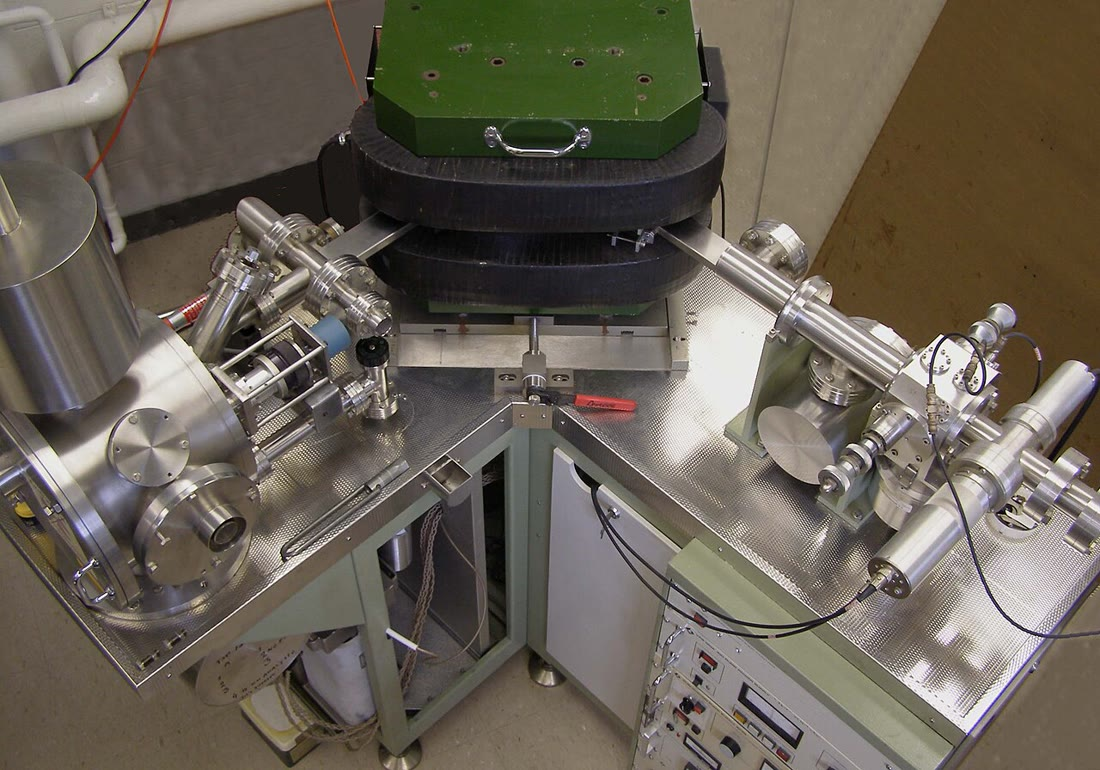
\includegraphics[width=0.42\linewidth]{images/book3/b1-tims.jpg}\hfill
\begin{minipage}[b]{0.55\linewidth}
يقيس مطياف كتلة الأيونات الحرارية (يسارًا) نِسَب النظائر لعناصر مثل السترونتيوم. يُفصل العنصر عن العيّنة المذابة بالكيمياء، ويُوضع على خيط معدني في فراغ؛ وحين يُسخَّن يطلق أيونات، تُسرَّع وتنحني بمجال المغناطيس الكبير (الملفّات السوداء في المركز)، فتنحني الأيونات الأخفّ أكثر من الأثقل، فيصل كل نظير إلى مجمّعه الخاص. ونِسَب النظائر هي ما يقيسه الجهاز أفضل ما يكون، ولهذا تكون الطرائق المبنية على النسب وحدها الأدقّ. (صورة: Radiogenic, CC0, عبر Wikimedia Commons.)
\end{minipage}
\end{inthelab}
% ledger: commons:tims, amherst:constants

\section{البوتاسيوم–الأرغون، واليورانيوم–الرصاص، والكربون المشع}\label{sec:b1:radiometric-methods:kar}

\subsection*{أصلٌ له ابنتان}

\begin{definition}[الاضمحلال المتفرّع]\label{def:b1:radiometric-methods:branching}
يخضع الأصل ل\emph{الاضمحلال المتفرّع}\index{الاضمحلال المتفرّع} حين تضمحلّ أنويته بطريقين أو أكثر إلى ابنات مختلفة. ولكل طريق $i$ ثابت اضمحلال جزئي $\lambda_i$ خاص به؛ ويضمحلّ الأصل بالثابت الكلّي $\lambda = \sum_i \lambda_i$، وينسلك كسر $\lambda_i/\lambda$ من الاضمحلالات الطريق~$i$. ويضمحلّ البوتاسيوم-40 إلى الكالسيوم-40 ب$\lambda_\beta =
\num{4.962e-10}$ لكل سنة، وإلى الأرغون-40 ب$\lambda_e = \num{0.581e-10}$ لكل سنة.
\end{definition}
% ledger: amherst:constants, iaea:k40-branches

\begin{proposition}[عمر البوتاسيوم–الأرغون]\label{prop:b1:radiometric-methods:kar}
\omterm{def:b1:rock-forming-minerals:mineral}{معدن} احتفظ بكل الأرغون الذي صُنع فيه، ولم يكن يحتوي شيئًا منه حين تبلّر، يحتوي بعد الزمن $t$
\[
  {}^{40}\mathrm{Ar}^* = \frac{\lambda_e}{\lambda}\;{}^{40}\mathrm{K}\,\bigl(e^{\lambda t} - 1\bigr),
  \qquad\text{أي}\qquad
  t = \frac{1}{\lambda}\,\ln\!\left(1 + \frac{\lambda}{\lambda_e}\,
      \frac{{}^{40}\mathrm{Ar}^*}{{}^{40}\mathrm{K}}\right),
\]
حيث ${}^{40}\mathrm{K}$ عدد ذرّات البوتاسيوم-40 اليوم، و$\lambda =
\lambda_\beta + \lambda_e$.
\end{proposition}

\begin{proof}
يضمحلّ الأصل بالثابت الكلّي $\lambda$ أيًّا كان الطريق، فبموجب \cref{prop:b1:radiometric-methods:growth} يكون عدد الاضمحلالات في الزمن $t$ هو ${}^{40}\mathrm{K}\,(e^{\lambda t} - 1)$. ويسلك كل اضمحلال طريق الأرغون باحتمال $\lambda_e/\lambda$، مستقلًّا عن الباقي؛ وعبر العدد الكبير جدًّا من الاضمحلالات يكون كسر ما أعطى أرغونًا هو $\lambda_e/\lambda$. وهذا يعطي ${}^{40}\mathrm{Ar}^*$؛ وحلّ المعادلة لأجل $t$ يعطي العمر.
\end{proof}

يحمل الأُسّ الثابت الكلّي، والعامل أمامه الثابت الجزئي: فاستعمال $\lambda_e$ في الأُسّ، كما لو كان الأرغون الطريق الوحيد، يعطي عمرًا خاطئًا بشدّة. ويحمل فرع الكالسيوم تسعة أعشار الاضمحلالات، لكنه غير مفيد للتأريخ، لأن الكالسيوم-40 هو النظير الشائع لعنصر وفير في الصخور؛ والأرغون، وهو غاز خامل، يهرب من المصهور، فيبدأ البلّور بقليل منه أو بلا شيء تقريبًا. والبوتاسيوم-40 يمثّل \qty{0.0117}{\percent} من ذرّات البوتاسيوم. وتحتاج الطريقة إلى الكميات المطلقة للبوتاسيوم والأرغون، تُقاس كلّ منهما على حدة. والأرغون الآتي من الهواء، الموجود في كل صخر، يُعرف بنظيره أرغون-36 ويُطرح بالنسبة الجوية $^{40}\mathrm{Ar}/^{36}\mathrm{Ar} = 295.5$.
% ledger: tulane:kar, iaea:k40-branches, amherst:constants, nmgrl:kar

تفشل الطريقة بطريقتين. فالأرغون الزائد يجعل الأعمار أقدم مما ينبغي: فالحمم التي تبرد بسرعة قد تحبس أرغونًا من \omterm{def:b1:layered-earth:layers}{الوشاح} في فقاعات، والحمم التاريخية تعطي عادةً أعمار بوتاسيوم–أرغون من 1 إلى 2 مليون سنة، وهو خطأ لا يهمّ إلا للصخور الفتية. وفقدان الأرغون يجعلها أحدث مما ينبغي: فمعظم \omterm{def:b1:rock-forming-minerals:mineral}{المعادن} تفقد الأرغون حين تُسخَّن فوق نحو \qty{300}{\celsius}، فيعيد تحوّل لاحق ضبط الساعة كليًّا أو جزئيًّا، ويعطي الفقدان الجزئي عمرًا بين الحدثين لا يؤرّخ أيًّا منهما. وتُفضَّل \omterm{def:b1:rock-forming-minerals:mineral}{المعادن} الغنية بالبوتاسيوم: السانيدين والبيوتايت، ثم \omterm{def:b1:rock-forming-minerals:groups}{البلاجيوكلاز} أو الهورنبلند.
% ledger: tulane:kar, nmgrl:kar

تقيس طريقة أرغون–أرغون النسب وحدها. تُعرَّض العيّنة لنيوترونات سريعة في قلب مفاعل نووي، بجوار \omterm{def:b1:rock-forming-minerals:mineral}{معدن} قياسي ذي عمر معلوم؛ فيحوّل التفاعل جزءًا من البوتاسيوم-39 إلى أرغون-39، فيقوم مقام البوتاسيوم، ويعطي المعيار مردود التفاعل. ويُقاس النظيران معًا في الغاز نفسه. ويمكن بعد ذلك تسخين العيّنة على مراحل، بفرن أو بليزر؛ فكل مرحلة تعطي عمرًا، وتُرسم الأعمار بدلالة الكسر التراكمي من الأرغون-39 المنطلق، فيكون ذلك طيف الأعمار. والمراحل المتّفقة ضمن أخطائها تشكّل هضبة؛ وطيف بلا هضبة يحذّر من أن \omterm{def:b1:rock-forming-minerals:mineral}{المعدن} لم يبقَ مغلقًا. وتزامن الاصطدام والانقراض عند نهاية الطباشيري يرتكز على أعمار أرغون–أرغون.
% ledger: amherst:arar, nmgrl:arar, renne:kpg

\subsection*{ساعتان يورانيّتان}

لليورانيوم نظيران طويلا العمر: اليورانيوم-238 يضمحلّ إلى الرصاص-206، واليورانيوم-235 إلى الرصاص-207، بمعدّلين مختلفين؛ واليوم $^{235}\mathrm{U}/^{238}\mathrm{U} = 0.0072567$، أي ذرّة واحدة من كل 137.8. \omterm{def:b1:rock-forming-minerals:mineral}{فمعدن} يحتوي اليورانيوم يحمل ساعتين مستقلّتين، لكل منهما معادلة نموّه الخاصة، ${}^{206}\mathrm{Pb}^* = {}^{238}\mathrm{U}\,(e^{\lambda_{238} t} - 1)$ و${}^{207}\mathrm{Pb}^* = {}^{235}\mathrm{U}\,(e^{\lambda_{235} t} - 1)$. فإن اتّفق العمران قيل إنهما متوافقان، والاتفاق اختبار أن \omterm{def:b1:rock-forming-minerals:mineral}{المعدن} بقي مغلقًا، وهذا ما لا تستطيعه ساعة واحدة. ويأتي التباين غالبًا من فقدان الرصاص من أجزاء من البلّورة أتلفها إشعاع اليورانيوم نفسه؛ ورسمٌ للنسبتين معًا، أي مخطط الكونكورديا، يستعيد عندئذٍ عمر البلّورة وعمر الحدث الذي جعلها تفقد الرصاص، وهي أداة من المجلد الثالث.
% ledger: amherst:constants, tulane:upb-zircon

الزركون، $\mathrm{ZrSiO_4}$، هو \omterm{def:b1:rock-forming-minerals:mineral}{المعدن} المختار: فهو يُدخل اليورانيوم إلى بنيته لكنه بالكاد يأخذ الرصاص، فيكون معظم رصاصه إشعاعيًّا؛ وهو صلب، يقاوم التجوية ويصمد أمام التحوّل، فتحتفظ الحبيبات المتآكلة من صخر بعمره في الرمال المشتقّة منه. ويُستعمل الأباتيت والسفين أيضًا، لكن أقلّ.
% ledger: tulane:upb-zircon, commons:zircon-cl

\subsection*{الكربون المشع}

يُصنع الكربون-14 باستمرار في الغلاف الجوي العلوي من النيتروجين-14 الذي تصدمه الأشعة الكونية. ويختلط بكربون الغلاف الجوي؛ والكائنات الحيّة تتبادل الكربون مع الجوّ وتحفظ نسبة الكربون-14 فيها. وعند الموت يتوقّف التبادل، ويضمحلّ الكربون-14 عائدًا إلى النيتروجين-14. وبما أن \omterm{def:b1:radiometric-methods:isochron}{النسبة الابتدائية} هي نسبة الجوّ، فإن العمر يتبع من قانون الاضمحلال وحده، دون إيزوكرون: $t = -\tau \ln(A/A_0)$، حيث $A$ نشاط كربون العيّنة، و$A_0$ نشاط الكربون الحيّ، و$\tau =
1/\lambda$ متوسط العمر. ويُؤرَّخ الخشب والفحم والعظم والأسنان والصدف بهذه الطريقة، حتى بضعة عشرات الآلاف من السنين: نحو \num{70000} سنة على الأكثر.
% ledger: tulane:c14, iaea:c14

\begin{definition}[عمر الكربون المشع، ومنحنى المعايرة]\label{def:b1:radiometric-methods:radiocarbon}
\emph{عمر الكربون المشع}\index{عمر الكربون المشع} (التقليدي) للعيّنة هو
\[
  t = -8033 \,\ln \frac{A_{\mathrm{SN}}}{A_{\mathrm{ON}}} \ \text{سنة BP},
\]
حيث $A_{\mathrm{SN}}$ نشاط كربون العيّنة و$A_{\mathrm{ON}}$ نشاط المعيار المرجعي؛ ويستعمل نصف عمر قدره \num{5568} سنة (متوسط عمر \num{8033} سنة)، ويُطبِّع النشاطات للتجزّؤ النظائري للكربون ($\delta^{13}\mathrm{C} = \qty{-25}{\permil}$)، ويعدّ السنين قبل عام 1950 م (BP، «قبل الحاضر»). و\emph{منحنى المعايرة}\index{منحنى المعايرة} يعطي عمر الكربون المشع لعيّنات ذات عمر تقويمي معروف؛ وإذا قُرئ بالعكس، يحوّل عمر الكربون المشع إلى مدى من الأعمار التقويمية (cal BP).
\end{definition}
% ledger: sp77:conventional-age, reimer20:intcal20

ليس \omterm{def:b1:radiometric-methods:radiocarbon}{عمر الكربون المشع} عمرًا بالسنين التقويمية، لسببين. فنصف العمر البالغ \num{5568} سنة، وهي قيمة ليبي المحفوظة اصطلاحًا، أقصر من ال\num{5700} سنة الحقيقية، فأعمار الكربون المشع تنقص نحو \qty{2.4}{\percent}. والأهمّ أن نسبة الكربون-14 في الجوّ لم تكن ثابتة. ويقيس \omterm{def:b1:radiometric-methods:radiocarbon}{منحنى المعايرة} الأثرين معًا، على أرشيفات مؤرّخة بشكل مستقلّ: حلقات الأشجار حتى نحو \num{13900} cal BP، وأبعد منها تسلسلات حلقات أشجار عائمة، ورواسب بحيرات وبحار، ورواسب كهوف ومرجان، حتى \num{55000} cal BP (الشكل أدناه).
% ledger: sp77:conventional-age, iaea:c14, reimer20:intcal20

\begin{omfigure}
\begin{tikzpicture}
\begin{axis}[name=main, omrecord, width=0.5\linewidth, height=6cm, xmin=0, xmax=12, ymin=0, ymax=12,
  xlabel={العمر التقويمي (ألف cal BP)}, ylabel={عمر الكربون المشع (ألف BP)},
  xtick={0,2,...,12}, ytick={0,2,...,12}]
% figdata/bachelor-1/radiocarbon.py, IntCal20 (dataset bachelor-1-intcal20); ledger: data:b3-intcal20
\addplot[black!50, dashed, domain=0:12, samples=2] {x};
\addplot[omDef, line width=0.9pt] table[x=cal, y=c14] {figdata/out/bachelor-1-radiocarbon-curve.dat};
\draw[omThm, line width=0.6pt] (axis cs:2.3,2.3) rectangle (axis cs:2.9,2.9);
\node[font=\scriptsize, anchor=east, text=black!60] at (axis cs:8.4,10.4) {أعمار متساوية};
\node[font=\scriptsize, text=omDef, anchor=north west] at (axis cs:7.4,5.6) {IntCal20};
\end{axis}
\begin{axis}[at={(main.east)}, anchor=west, xshift=2.1cm, omrecord, width=0.38\linewidth, height=6cm,
  xmin=2300, xmax=2900, ymin=2300, ymax=2900, xlabel={العمر التقويمي (cal BP)}, ylabel={عمر الكربون المشع (BP)},
  xtick={2300,2500,2700,2900}, ytick={2300,2500,2700,2900},
  x tick label style={/pgf/number format/.cd, set thousands separator={}},
  y tick label style={/pgf/number format/.cd, set thousands separator={}}]
\addplot[name path=hi, draw=none, forget plot] table[x=cal, y=hi] {figdata/out/bachelor-1-radiocarbon-zoom.dat};
\addplot[name path=lo, draw=none, forget plot] table[x=cal, y=lo] {figdata/out/bachelor-1-radiocarbon-zoom.dat};
\addplot[omDef!25, forget plot] fill between[of=hi and lo];
\addplot[omDef, line width=0.8pt] table[x=cal, y=c14] {figdata/out/bachelor-1-radiocarbon-zoom.dat};
\addplot[omThm, line width=0.6pt, domain=2300:2900, samples=2] {2480};
\draw[omThm, densely dotted] (axis cs:2495,2300) -- (axis cs:2495,2480);
\draw[omThm, densely dotted] (axis cs:2699,2300) -- (axis cs:2699,2480);
\node[font=\scriptsize, text=omThm, anchor=south west] at (axis cs:2310,2485) {$2480$ BP};
\end{axis}
\end{tikzpicture}

{\small يسارًا: \omterm{def:b1:radiometric-methods:radiocarbon}{منحنى المعايرة} IntCal20 على مدى آخر \num{12000} سنة، \omterm{def:b1:radiometric-methods:radiocarbon}{عمر الكربون المشع} بدلالة العمر التقويمي؛ والخط المتقطّع هو المكان الذي يتساوى فيه العمران. ويمينًا: الصندوق الأيسر مكبّرًا، مع نطاق عدم يقين معياري واحد للمنحنى. وبين \num{2500} و\num{2700} cal BP يكون المنحنى شبه مسطّح: فعمر كربون مشع قدره 2480 سنة BP يطابق أعمارًا تقويمية من نحو \num{2495} إلى \num{2699} cal BP.}
\label{fig:b1:radiometric-methods:intcal}
\end{omfigure}
% ledger: data:b3-intcal20, reimer20:intcal20

عند \num{2000} cal BP يعطي المنحنى \num[uncertainty-mode=separate]{2070 \pm 14} سنة BP؛ وعند \num{12000} cal BP، \num{10306}: فأعمار الكربون المشع هناك أصغر ب\num{1694} سنة من الأعمار التقويمية، وهو أكبر بكثير من \qty{2.4}{\percent} من نصف العمر. والمنحنى يتموّج، وحيث يكون مسطّحًا يطابق عمر كربون مشع مدًى طويلًا من الأعمار التقويمية، مهما كان القياس دقيقًا.
% ledger: data:b3-intcal20

\begin{dated}{2020}
% ledger: reimer20:intcal20
المنحنى المستعمل للنصف الشمالي هو IntCal20، المنشور عام 2020. وقد حلّ محلّ IntCal13، مضيفًا بيانات جديدة ومدًّا للمنحنى حتى \num{55000} cal BP، مع منحنيات منفصلة للنصف الجنوبي وسطح المحيط. وتُراجَع منحنيات المعايرة كلّما قيست أرشيفات جديدة، فيجب أن يذكر العمر التقويمي المنحنى الذي أنتجه.
\end{dated}

\section{درجة الإغلاق}\label{sec:b1:radiometric-methods:closure}

لا يبدأ \omterm{def:b1:rock-forming-minerals:mineral}{المعدن} الذي يتبلّر من ماجما عند \qty{800}{\celsius} ساعته فورًا. فبينما هو حارّ، تنتشر ذرّات الابنة، والأرغون بالدرجة الأولى، عبر شبكته البلّورية وتهرب؛ ولا يصير الانتشار بطيئًا بما يكفي ليُهمل إلا حين يبرد بما يكفي، فتبدأ الابنة بالتراكم.
% ledger: leeds:closure, tulane:kar, tulane:magma-types

\begin{definition}[درجة الإغلاق، وعمر التبريد]\label{def:b1:radiometric-methods:closure}
\emph{درجة الإغلاق}\index{درجة الإغلاق} \omterm{def:b1:rock-forming-minerals:mineral}{لمعدن} من أجل نظام اضمحلال هي الحرارة التي تحتها لا تنتشر ذرّات الأصل والابنة داخل شبكته أو خارجها بسرعة تكفي لتكون ذات أهمية، فيسلك \omterm{def:b1:rock-forming-minerals:mineral}{المعدن} سلوك نظام مغلق. و\emph{عمر التبريد}\index{عمر التبريد} عمر يُقاس في \omterm{def:b1:rock-forming-minerals:mineral}{معدن} تكوّن فوق درجة إغلاقه: فهو يؤرّخ اللحظة التي برد فيها \omterm{def:b1:rock-forming-minerals:mineral}{المعدن} عبر تلك الدرجة، لا اللحظة التي تكوّن فيها.
\end{definition}
% ledger: leeds:closure

تختلف \omterm{def:b1:radiometric-methods:closure}{درجات الإغلاق} من \omterm{def:b1:rock-forming-minerals:mineral}{معدن} إلى آخر لاختلاف الشبكات، ومن عنصر إلى آخر لأن الذرّات المختلفة تنتشر عبر الشبكة نفسها بسرعات مختلفة (الشكل أدناه). وهي تقريبية: فجدولان يعطيان \qty{280}{\celsius} و\qty{350}{\celsius} للأرغون في البيوتايت، و\qty{530}{\celsius} و\qty{550}{\celsius} للأرغون في الهورنبلند. وآثار الانشطار، وهي آثار الضرر الذي يتركه في البلّورة الانشطار التلقائي لأنوية اليورانيوم، تلتئم عند درجات أدنى حتى من ذلك.
% ledger: leeds:closure, amherst:closure

\begin{omfigure}
\begin{tikzpicture}
\begin{axis}[width=0.8\linewidth, height=7cm, xbar, bar width=7pt, xmin=0, xmax=850,
  xlabel={درجة الإغلاق (\unit{\celsius})},
  symbolic y coords={zrupb,spupb,hbar,mssr,msar,btsr,btar,zrft,kfsar,apft},
  ytick={zrupb,spupb,hbar,mssr,msar,btsr,btar,zrft,kfsar,apft}, y dir=reverse, enlarge y limits=0.07,
  yticklabels={{الزركون، U--Pb},{السفين، U--Pb},{الهورنبلند، K--Ar},{الموسكوفيت، Rb--Sr},{الموسكوفيت، K--Ar},{البيوتايت، Rb--Sr},{البيوتايت، K--Ar},{الزركون، آثار الانشطار},{فلسبار البوتاسيوم، K--Ar},{الأباتيت، آثار الانشطار}},
  y tick label style={font=\scriptsize}, x tick label style={font=\scriptsize},
  axis x line*=bottom, axis y line*=left]
% ledger: leeds:closure (values as tabulated; > lower bound, ~ approximate, ranges and +- as given)
\addplot[fill=omDef!55, draw=omDef, error bars/.cd, x dir=both, x explicit]
  coordinates {(750,zrupb) (650,spupb) (530,hbar) +- (40,0) (500,mssr) (350,msar) (320,btsr)
               (280,btar) +- (40,0) (200,zrft) +- (25,0) (130,kfsar) (105,apft) +- (10,0)};
\node[font=\scriptsize, anchor=west] at (axis cs:755,zrupb) {$> 750$};
\node[font=\scriptsize, anchor=west] at (axis cs:655,spupb) {$> 650$};
\node[font=\scriptsize, anchor=west] at (axis cs:575,hbar) {$530 \pm 40$};
\node[font=\scriptsize, anchor=west] at (axis cs:505,mssr) {$500$};
\node[font=\scriptsize, anchor=west] at (axis cs:355,msar) {$\approx 350$};
\node[font=\scriptsize, anchor=west] at (axis cs:325,btsr) {$320$};
\node[font=\scriptsize, anchor=west] at (axis cs:325,btar) {$280 \pm 40$};
\node[font=\scriptsize, anchor=west] at (axis cs:230,zrft) {$175$--$225$};
\node[font=\scriptsize, anchor=west] at (axis cs:135,kfsar) {$\approx 130$، متسرّب};
\node[font=\scriptsize, anchor=west] at (axis cs:120,apft) {$105 \pm 10$};
\end{axis}
\end{tikzpicture}

{\small \omterm{def:b1:radiometric-methods:closure}{درجات الإغلاق} لأهمّ ساعات \omterm{def:b1:rock-forming-minerals:mineral}{المعادن}، من جدول منشور واحد. U--Pb هو اليورانيوم–الرصاص، وK--Ar البوتاسيوم–الأرغون (والأرغون–أرغون)، وRb--Sr الروبيديوم–السترونتيوم. وبالنسبة إلى آثار الانشطار تكون القيمة درجة الحرارة التي تلتئم عندها الآثار.}
\label{fig:b1:radiometric-methods:closure}
\end{omfigure}

وفي كتلة صهارية بطيئة التبريد تُغلق الساعات واحدة بعد الأخرى، من الأشدّ حرارة إلى الأبرد: الزركون أولًا، قرب تبلّره، ثم الهورنبلند، ثم الموسكوفيت والبيوتايت. وتفرّق أعمارها يسجّل التبريد.

\begin{proposition}[معدّل التبريد بين درجتي إغلاق]\label{prop:b1:radiometric-methods:cooling}
إذا أعطى معدنان من صخر واحد، ذوا \omterm{def:b1:radiometric-methods:closure}{درجتي إغلاق} $T_1 > T_2$، \omterm{def:b1:radiometric-methods:closure}{أعمار تبريد} $t_1 > t_2$، فإن متوسط معدّل التبريد بين الإغلاقين هو
\[
  \dot T = \frac{T_1 - T_2}{t_1 - t_2}.
\]
وإن كان الصخر على عمق ترتفع فيه الحرارة مع العمق بانحدار ثابت $G$ تحت سطح عند الحرارة $T_s$، فقد كان على العمق $z_i
= (T_i - T_s)/G$ حين أُغلقت الساعة $i$.
\end{proposition}

\begin{proof}
كان الصخر عند $T_1$ في الزمن $t_1$، وعند $T_2$ في الزمن $t_2$؛ ومتوسط معدّل تغيّر حرارته هو نسبة الفرقين. ومع منحنًى حراري خطّي (\cref{def:b1:heat-budget:geotherm})، $T = T_s + G z$، وهذا يعطي العمق.
\end{proof}

يعطي العمق معدّل \omterm{def:b1:geological-maps:geological-map}{انكشاف} بمجرّد معرفة الزمن الذي وصل فيه الصخر إلى السطح، كما في مسألة هذا الفصل. والطريقة خشنة: \omterm{def:b1:radiometric-methods:closure}{فدرجات الإغلاق} غير مؤكّدة بعشرات الدرجات، \omterm{def:b1:heat-budget:geotherm}{والمنحنى الحراري} يُفترض ثابتًا عبر الزمن. أما التأريخ الحراري، أي إعادة بناء مسارات الحرارة–الزمن تفصيليًّا من ساعات كثيرة، فهو موضوع المجلد الثالث.

\section{تأريخ المتتاليات الرسوبية}\label{sec:b1:radiometric-methods:sediments}

أغلب الصخور الرسوبية لا يمكن تأريخها مباشرة. فحبيباتها أقدم من الصخر: فحبيبة زركون فُتاتية، كالحبيبة في مقدّمة هذا الفصل، تؤرّخ الصخر الذي تآكلت منه. والكربون المشع يؤرّخ المادة العضوية الفتية فقط. لذلك تأتي أعمار المخطّط من صخور تبلّرت لحظة ترسيبها، أي رماد بركاني وتدفّقات حمم داخل التتابع، ومن صخور نارية تقطعه.
% ledger: tulane:upb-zircon, tulane:c14, commons:zircon-cl

\begin{definition}[العمر الحاصر]\label{def:b1:radiometric-methods:bracketing}
\emph{العمر الحاصر}\index{العمر الحاصر} هو حدّ يُوضع على عمر مستوى رسوبي بصخور مؤرَّخة مرتبطة به بمبادئ علم الطبقات: عمر أقصى من طبقة مؤرّخة تحته، أو من أحدث حبيبة فُتاتية فيها؛ وعمر أدنى من طبقة مؤرّخة فوقه، أو من تداخل يقطعه. والمستوى الواقع بين أقصى وأدنى يكون محصورًا.
\end{definition}

\begin{omfigure}
\begin{tikzpicture}[x=1cm, y=0.62cm]
  % column
  \fill[lith shale] (0,0) rectangle (2.4,3);
  \fill[lith sandstone] (0,3) rectangle (2.4,6);
  \fill[lith shale] (0,6) rectangle (2.4,9);
  \fill[lith limestone] (0,9) rectangle (2.4,12);
  \draw (0,0) rectangle (2.4,12);
  % ash bed below, lava flow above
  \fill[omThm!70] (0,2.0) rectangle (2.4,2.3);
  \fill[black!65] (0,9.0) rectangle (2.4,9.6);
  % boundary
  \draw[omDef, line width=1.2pt] (-0.3,7.2) -- (2.7,7.2);
  % dyke cutting everything
  \fill[black!40] (1.55,0) -- (1.85,0) -- (1.95,12) -- (1.65,12) -- cycle;
  % detrital zircons
  \foreach \p in {(0.4,3.6),(0.9,4.5),(0.5,5.4),(1.2,3.9),(0.8,5.0)}
    \fill[omThm] \p circle (1.3pt);
  % labels
  \node[anchor=west, font=\small, align=left] at (3.0,2.15) {طبقة رماد، $t_1$: عمر أقصى};
  \node[anchor=west, font=\small, align=left] at (3.0,4.5) {أحدث حبيبة زركون فُتاتية، $t_0$:\\عمر أقصى للحجر الرملي};
  \node[anchor=west, font=\small, text=omDef] at (3.0,7.2) {المستوى المراد تأريخه};
  \node[anchor=west, font=\small, align=left] at (3.0,9.3) {تدفّق حمم، $t_2$: عمر أدنى};
  \node[anchor=west, font=\small, align=left] at (3.0,11.3) {دايك، $t_3$: عمر أدنى لكل\\طبقة يقطعها};
  \draw[black!50] (2.5,2.15) -- (2.95,2.15);
  \draw[black!50] (1.25,4.5) -- (2.95,4.5);
  \draw[black!50] (2.5,9.3) -- (2.95,9.3);
  \draw[black!50] (1.95,11.3) -- (2.95,11.3);
\end{tikzpicture}

{\small أعمار تحصر مستوى في تتابع رسوبي (تخطيطي). فطبقة الرماد تحته، وأحدث الزركونات الفُتاتية في الحجر الرملي، تعطيان أعمارًا قصوى؛ والتدفّق البركاني فوقه، والدايك الذي يقطع التتابع كلّه، يعطيان أعمارًا دنيا. والمستوى أحدث من $t_1$ وأقدم من $t_2$؛ والدايك لا يضيف إلا أنه أقدم من $t_3$.}
\label{fig:b1:radiometric-methods:bracketing}
\end{omfigure}

أفضل الحصرات قريبة ودقيقة: طبقتا رماد تبعدان بضعة أمتار، مؤرّختان على الزركون بدقّة بضعة عشرات الآلاف من السنين، مع استكمال المستوى بينهما ب\cref{prop:b1:stratigraphic-scale:interpolation}. وفي مَيشان يقع GSSP لقاعدة الترياسي بين خمس طبقات رماد مؤرّخة؛ ويُحصر الانقراض بين \qty[uncertainty-mode=separate]{251.941(37)}{\Ma} و\qty[uncertainty-mode=separate]{251.880(31)}{\Ma}، وتُوضع قاعدة \omterm{def:b1:stratigraphic-scale:chronostratigraphy}{النظام} عند \qty[uncertainty-mode=separate]{251.902(24)}{\Ma} (\cref{sec:b1:stratigraphic-scale:extinctions}). وطبقات الرماد، التي تحملها الرياح عبر السحنات، هي في آن واحد خطوط زمن وساعات.
% ledger: burgess:end-permian, gssp:induan, ics:base.Triassic

المخطّط ليس أدقّ من الطبقات المؤرّخة قرب كلّ حدّ. فقاعدة الترياسي معروفة بدقّة \qty{0.024}{\Myr}، أي جزء من عشرة آلاف؛ وقاعدة الكربوني بدقّة \qty{0.19}{\Myr}؛ وقاعدة الديفوني بدقّة \qty{1.36}{\Myr}. وحيث لا تقع طبقة مؤرّخة قرب حدّ، يُستكمل عمره بين طبقات بعيدة، ويكبر عدم يقينه بقدر ذلك. وكل طبقة رماد جديدة تُؤرَّخ قرب حدّ يمكن أن تحرّكه، ولهذا يحمل المخطّط تاريخ نسخة.
% ledger: ics:base.Triassic, ics:base.Carboniferous, gssp:lochkovian

\section{التمارين}

\begin{exercise}[$\star$]\label{exo:b1:radiometric-methods:1}
(أ)~\omterm{def:b1:rock-forming-minerals:mineral}{معدن} يحتوي ثلاثة أضعاف من ذرّات \omterm{def:b1:radiometric-methods:radiogenic}{الابنة الإشعاعية} بالنسبة إلى ذرّات الأصل. كم نصف عمر يبلغ عمره؟ (ب)~احسب $D^*/P$ بعد \qty{310}{\Myr} للروبيديوم-87 ولليورانيوم-235، بالثوابت الواردة في \cref{tab:b1:radiometric-methods:systems}. أيّ النسبتين أسهل قياسًا بدقّة؟ (ج)~بعد كم نصف عمر لا يبقى من الأصل إلا أقلّ من \qty{1}{\percent}؟
% ledger: villa22:rb87, amherst:constants
\end{exercise}

\begin{exercise}[$\star$]\label{exo:b1:radiometric-methods:2}
أيّ طريقة من \cref{tab:b1:radiometric-methods:systems} تستعمل، وعلى أيّ مادة، لتأريخ: (أ)~فحم من موقد عمره نحو \num{8000} سنة؛ (ب)~طبقة رماد يُظنّ أن عمرها نحو \qty{66}{\Ma}، غنيّة بالسانيدين والزركون؛ (ج)~جرانيت عمره نحو \qty{2.7}{\Ga}؛ (د)~صدفة عمرها نحو \num{40000} سنة؛ (ه)~حجر كلسي من الجوراسي لا توجد فيه طبقة بركانية؟
% ledger: tulane:c14, tulane:kar, tulane:upb-zircon
\end{exercise}

\begin{exercise}[$\star$]\label{exo:b1:radiometric-methods:3}
الكربون في قطعة من الخشب له ربع نشاط المعيار، بعد التطبيع. (أ)~احسب \omterm{def:b1:radiometric-methods:radiocarbon}{عمر الكربون المشع} التقليدي. (ب)~احسب عمره بنصف العمر البالغ \num{5700} سنة. (ج)~لماذا لا يكون أيّ منهما عمرها بالسنين التقويمية، وكيف يُحصل على ذلك العمر؟
% ledger: sp77:conventional-age, iaea:c14
\end{exercise}

\begin{exercise}[$\star$]\label{exo:b1:radiometric-methods:4}
يعطي غرانيت عمرًا باليورانيوم–الرصاص على الزركون قدره \qty{420}{\Ma}، وعمرًا بالبوتاسيوم–الأرغون على الهورنبلند قدره \qty{410}{\Ma}، وعلى البيوتايت \qty{398}{\Ma}. (أ)~لماذا تختلف الأعمار الثلاثة، وبهذا الترتيب؟ (ب)~\omterm{def:b1:radiometric-methods:closure}{بدرجات الإغلاق} الواردة في شكل \cref{sec:b1:radiometric-methods:closure}، احسب متوسط معدّل التبريد بين إغلاقي الهورنبلند والبيوتايت. (ج)~ماذا يمكن أن يقال عن معدّل التبريد بين إغلاق الزركون وإغلاق الهورنبلند؟
% ledger: leeds:closure
\end{exercise}

\begin{exercise}[$\star\star$]\label{exo:b1:radiometric-methods:5}
أربع عيّنات صخرية كاملة من صخر النيس (بيانات تمرين) تعطي $^{87}\mathrm{Rb}/^{86}\mathrm{Sr} = 2.0$، $5.0$، $9.0$، $14.0$ و$^{87}\mathrm{Sr}/^{86}\mathrm{Sr} = 0.7323$، $0.7741$، $0.8307$، $0.9010$. (أ)~ركّب خطّ المربّعات الصغرى بطريقة \cref{met:b1:radiometric-methods:isochron}. (ب)~احسب العمر \omterm{def:b1:radiometric-methods:isochron}{والنسبة الابتدائية}. (ج)~احسب $s$ وعدم يقين العمر. (د)~هل تشير \omterm{def:b1:radiometric-methods:isochron}{النسبة الابتدائية} إلى مصدر في \omterm{def:b1:layered-earth:layers}{الوشاح} أم في \omterm{def:b1:layered-earth:layers}{القشرة}؟
% ledger: villa22:rb87, tulane:sr-initial
\end{exercise}

\begin{exercise}[$\star\star$]\label{exo:b1:radiometric-methods:6}
يحتوي سانيدين من طبقة رماد على \qty{10.0}{\percent} بوتاسيوم بالكتلة، و\qty{1.169}{nmol} من الأرغون-40 الإشعاعي لكل غرام. (أ)~بالوزن الذري للبوتاسيوم، \qty{39.098}{g.mol^{-1}}، ووفرة البوتاسيوم-40، احسب عدد مولات البوتاسيوم-40 لكل غرام. (ب)~احسب عمر البوتاسيوم–الأرغون. (ج)~لو كان \qty{0.5}{\percent} من الأرغون المقاس قد حُبس حين سقط الرماد، لا صُنع بالاضمحلال، فبكم يكون العمر أقدم من الواقع؟ هل يُقلق هذا هنا؟
% ledger: ciaaw:K, iaea:k40-branches, amherst:constants, tulane:kar
\end{exercise}

\begin{exercise}[$\star\star$]\label{exo:b1:radiometric-methods:7}
يعطي منحنى IntCal20 أعمار الكربون المشع \num[uncertainty-mode=separate]{2070 \pm 14} سنة BP عند \num{2000} cal BP، و\num{7178} عند \num{8000} cal BP، و\num{10306} عند \num{12000} cal BP. (أ)~بذرة تعطي \num[uncertainty-mode=separate]{2070 \pm 14} سنة BP. ما عمرها التقويمي؟ (ب)~وأخرى تعطي \num[uncertainty-mode=separate]{2480 \pm 15} سنة BP؛ وباستعمال اللوحة اليمنى من شكل \cref{sec:b1:radiometric-methods:kar}، أعطِ مدى أعمارها التقويمية، ووضّح لماذا يكون واسعًا إلى هذا الحدّ. (ج)~بكم سنة، وفي أيّ اتجاه، تختلف أعمار الكربون المشع عن الأعمار التقويمية عند \num{2000} و\num{8000} و\num{12000} cal BP؟ هل يكبر الفرق بنسبة إلى العمر؟
% ledger: data:b3-intcal20
\end{exercise}

\begin{exercise}[$\star\star$]\label{exo:b1:radiometric-methods:8}
في قطاع بحري يُؤرَّخ رماد عند \qty{4}{m} ب\qty[uncertainty-mode=separate]{94.50(10)}{\Ma}، وتدفّق حمم عند \qty{20}{m} ب\qty[uncertainty-mode=separate]{93.80(12)}{\Ma}؛ ودايك يقطع القطاع كلّه يُؤرَّخ ب\qty[uncertainty-mode=separate]{93.20(8)}{\Ma}. وأحدث زركون فُتاتي في حجر رملي عند \qtyrange{6}{10}{m} هو \qty[uncertainty-mode=separate]{95.3(4)}{\Ma}. ويُوضع حدّ طابق عند \qty{12}{m}. (أ)~أيّ الأعمار الأربعة تحصر الحدّ، وأيّها لا فائدة منه له؟ (ب)~استكمل عمره وعدم يقينه ب\cref{prop:b1:stratigraphic-scale:interpolation}. (ج)~ماذا يخبرنا الزركون الفُتاتي عن الحجر الرملي؟
\end{exercise}

\begin{exercise}[$\star\star$]\label{exo:b1:radiometric-methods:9}
يعطي زركونان من غرانيت واحد $^{206}\mathrm{Pb}^*/^{238}\mathrm{U} = 0.08401$ و$^{207}\mathrm{Pb}^*/^{235}\mathrm{U} = 0.6688$ (الحبّة~A)، و$0.05881$ و$0.4682$ (الحبّة~B). (أ)~احسب العمرين لكل حبّة. (ب)~أيّ الحبّتين متوافقة؟ (ج)~فقدت الحبّة~B جزءًا من رصاصها مؤخرًا. بيّن أن نسبتيها كلتيهما هما \qty{70}{\percent} من نسبتي الحبّة~A، ووضّح لماذا يختلف عمراها رغم أن الفقدان كان واحدًا للنظيرين.
% ledger: amherst:constants, tulane:upb-zircon
\end{exercise}

\begin{exercise}[$\star\star\star$]\label{exo:b1:radiometric-methods:10}
(أ)~بيّن أنه حين يكون $\lambda t \ll 1$ تُختزل معادلة العمر إلى $t \approx
(D^*/P)/\lambda$، وأن الخطأ النسبي لهذا التقريب قريب من $\lambda t/2$. (ب)~احسب الخطأ للروبيديوم-87 عند \qty{310}{\Ma}، وللبوتاسيوم-40 عند \qty{296}{\Ma}، ولليورانيوم-238 عند \qty{4.4}{\Ga}. (ج)~إذا قيست $D^*/P$ بدقّة \qty{0.1}{\percent}، فما عدم يقين عمر روبيديوم–سترونتيوم قدره \qty{310}{\Ma}؟
% ledger: villa22:rb87, amherst:constants
\end{exercise}

\begin{exercise}[$\star\star\star$]\label{exo:b1:radiometric-methods:11}
تبلّر البيوتايت وأُغلق منذ \qty{400}{\Myr}. وقبل \qty{200}{\Myr} أدّى تسخين وجيز إلى فقدانه كسرًا $f$ من أرغونه، وبعدها أُغلق من جديد. (أ)~بيّن أنه اليوم
\[
  \frac{\lambda}{\lambda_e}\,\frac{^{40}\mathrm{Ar}^*}{^{40}\mathrm{K}} =
  (1 - f)\bigl(e^{\lambda t_1} - e^{\lambda t_2}\bigr) + e^{\lambda t_2} - 1,
\]
مع $t_1 = \qty{400}{\Myr}$ و$t_2 = \qty{200}{\Myr}$. (ب)~احسب عمر البوتاسيوم–الأرغون الظاهري من أجل $f = 0$، و$0.3$، و$0.6$ و$1$. (ج)~لماذا لا يستطيع عمر بوتاسيوم–أرغون واحد أن يميّز الفقدان الجزئي من حدث أحدث؟
% ledger: amherst:constants, tulane:kar
\end{exercise}

\begin{exercise}[$\star\star\star$]\label{exo:b1:radiometric-methods:12}
عند \num{12000} cal BP يعطي منحنى IntCal20 عمر كربون مشع قدره \num{10306} سنة BP. (أ)~أعِد حساب العمر من نسبة النشاط نفسها بنصف عمر \num{5700} سنة. (ب)~كم من ال\num{1694} سنة التي يقصر بها \omterm{def:b1:radiometric-methods:radiocarbon}{عمر الكربون المشع} عن العمر التقويمي تفسّره اصطلاحية نصف العمر؟ (ج)~بافتراض أن الباقي يأتي من نسبة أعلى للكربون-14 في الجوّ قبل \num{12000} سنة، احسب بكم بالمئة تجاوزت هذه النسبة نسبة المعيار.
% ledger: data:b3-intcal20, sp77:conventional-age, iaea:c14
\end{exercise}

\section{مسألة: تأريخ غرانيت فاردن وغطائه}

\begin{problem}[{مسألة نهاية الأسبوع --- كيف تؤرّخ أربع ساعات تبلّر الغرانيت وتبريده وانكشافه}]
\label{pb:b1:radiometric-methods:1}
% values: calc/ch25.py; the analyses are invented, consistent with the Varden granite of 310 Ma (region.py)
يتداخل غرانيت تلال فاردن، المنطقة الخيالية للسلسلة، في قاعدة من الشيست، ويعلوه، فوق \omterm{def:b1:cross-sections:unconformity}{عدم التوافق}، الحجر الرملي الترياسي. استعمل ثوابت \cref{tab:b1:radiometric-methods:systems}، \omterm{def:b1:radiometric-methods:closure}{ودرجات الإغلاق} في شكل \cref{sec:b1:radiometric-methods:closure}، والوزن الذري للبوتاسيوم \qty{39.098}{g.mol^{-1}}، ووفرة البوتاسيوم-40، \qty{0.0117}{\percent} من ذرّات البوتاسيوم. وجميع التحاليل بيانات تمرين.

\medskip
\noindent\textbf{الجزء الأول --- إيزوكرون لصخر كامل.} تعطي ست عيّنات صخرية كاملة:
\begin{center}
\small
\begin{tabular}{|l|cccccc|}
\hline
$^{87}\mathrm{Rb}/^{86}\mathrm{Sr}$ & 0.92 & 2.15 & 3.40 & 5.05 & 7.60 & 10.30 \\
$^{87}\mathrm{Sr}/^{86}\mathrm{Sr}$ & 0.71211 & 0.71718 & 0.72284 & 0.72986 & 0.74113 & 0.75261 \\
\hline
\end{tabular}
\end{center}
\begin{enumerate}
  \item ارسم العيّنات الست. هل تقع على خطّ مستقيم؟
  \item احسب $\bar x$ و$\bar y$ و$S_{xx}$ و$S_{xy}$، ثم ميل المربّعات الصغرى.
  \item احسب القطع. ماذا يمثّل؟
  \item احسب عمر الغرانيت.
  \item احسب البواقي و$s$، وعدم يقين العمر.
  \item هل تقترب \omterm{def:b1:radiometric-methods:isochron}{النسبة الابتدائية} من نسبة \omterm{def:b1:layered-earth:layers}{الوشاح} أم من نسبة \omterm{def:b1:layered-earth:layers}{القشرة} القارية؟ لو كانت الصهارة مزيجًا من مصهورين بنسبتي $0.7025$ و$0.710$، متساويين في غناهما بالسترونتيوم، فأيّ حصّة من سترونتيومها جاءت من \omterm{def:b1:layered-earth:layers}{القشرة}؟
\end{enumerate}

\noindent\textbf{الجزء الثاني --- البوتاسيوم والأرغون.} يحتوي بيوتايت على \qty{7.40}{\percent} بوتاسيوم بالكتلة و\qty{4.139}{nmol} من الأرغون-40 الإشعاعي لكل غرام؛ والهورنبلند \qty{1.10}{\percent} و\qty{0.6333}{nmol.g^{-1}}.
\begin{enumerate}[resume]
  \item احسب عدد ذرّات البوتاسيوم-40 في غرام من البيوتايت.
  \item احسب عمر البوتاسيوم–الأرغون للبيوتايت.
  \item احسب عمر الهورنبلند.
  \item ما العمر الذي كان سيعطيه البيوتايت لو نُسي التفرّع، وعُدّت كل الاضمحلالات أرغونًا؟ ولماذا لا يُستعمل الكالسيوم-40 بدلًا منه؟
  \item لماذا لا يُقلق هنا الأرغون الزائد المحبوس حين تكوّنت \omterm{def:b1:rock-forming-minerals:mineral}{المعادن}؟
  \item كلا العمرين أحدث من عمر \omterm{def:b1:radiometric-methods:isochron}{الإيزوكرون}. أعطِ تفسيرين، ووضّح كيف يمكن لطيف عمر أرغون–أرغون أن يميّز بينهما.
\end{enumerate}

\noindent\textbf{الجزء الثالث --- التبريد.} يعطي زركون من الغرانيت $^{206}\mathrm{Pb}^*/^{238}\mathrm{U} = 0.049361$ و$^{207}\mathrm{Pb}^*/^{235}\mathrm{U} = 0.35784$.
\begin{enumerate}[resume]
  \item احسب عمري اليورانيوم–الرصاص. هل هما متوافقان؟
  \item انسب كل عمر من الأجزاء الأول إلى الثالث إلى الحدث الذي يؤرّخه. ارسم حرارة الغرانيت بدلالة الزمن من الزركون إلى البيوتايت.
  \item احسب متوسط معدّل التبريد بين إغلاقي الهورنبلند والبيوتايت.
  \item ماذا يمكن أن يقال عن معدّل التبريد بين إغلاق الزركون وإغلاق الهورنبلند؟
  \item بعدم يقين قدره \qty{40}{\celsius} على كل من \omterm{def:b1:radiometric-methods:closure}{درجتي الإغلاق}، مستقلّتين، فما مدى معدّلات التبريد الممكنة؟
  \item بالجدول الآخر المذكور في الفصل (\qty{550}{\celsius} للهورنبلند، و\qty{350}{\celsius} للبيوتايت)، ما المعدّل الذي يُوجد؟ ماذا يقول هذا عن النتيجة؟
  \item افترض منحنًى حراريًّا قدره \qty{30}{\celsius.km^{-1}} تحت سطح عند \qty{10}{\celsius}. على أيّ عمق كان الغرانيت حين أُغلق البيوتايت؟
\end{enumerate}

\noindent\textbf{الجزء الرابع --- \omterm{def:b1:cross-sections:unconformity}{عدم التوافق}.} طبقة رماد على \qty{18}{m} فوق قاعدة الحجر الرملي الترياسي تحوي زركونات بنسبتين $^{206}\mathrm{Pb}^*/^{238}\mathrm{U} = 0.039108$ و$^{207}\mathrm{Pb}^*/^{235}\mathrm{U} = 0.27577$. وطبقة رماد ثانية، على \qty{58}{m} فوق القاعدة، مؤرّخة ب\qty{245.30}{\Ma}. وتعطي زركونات فُتاتية في أدنى متر من الحجر الرملي أعمارًا حول \qty{310}{\Ma}.
\begin{enumerate}[resume]
  \item احسب عمر طبقة الرماد السفلى.
  \item من أين تأتي الزركونات الفُتاتية، وماذا تقول عن عمر الحجر الرملي؟
  \item احسب معدّل تراكم الحجر الرملي بين طبقتي الرماد، وعمر قاعدته، بافتراض المعدّل نفسه تحت الرماد السفلى.
  \item كم تطول الفجوة في السجلّ عند \omterm{def:b1:cross-sections:unconformity}{عدم التوافق}، من تبلّر الغرانيت إلى ترسيب الحجر الرملي؟
  \item احسب متوسط معدّل التآكل الذي أوصل الغرانيت من عمق سؤال~19 إلى السطح. ما الافتراض الذي يفرضه هذا بشأن المكان الذي كان فيه الغرانيت المتآكل؟
  \item ما معدّل تبريد الغرانيت؟
\end{enumerate}
\end{problem}
